\chapter{Exercise 1. Your first project}
We will create an application based in the concept “Gamify Your Life”. The main idea is to divide the life in 3 sections, Health, Work and Social Relationships. Inside those section we can find different user targets for each day.
\section{-}
With the option “Start new Android Studio Project” or getting the option “File->New project”, you must create a new project. From this you must choose the “Empty Views Activity”.
\section{-}
Next you need to configure the project with the following parameters.
\\ \\
Name: “Name you want to use”\\
Package name: edu.urv.”name of your app” Location: your location\\
Language: Java Minimum\\
SDK: API 27\\
Build Configuration Language: Kotlin DSI\\
\section{Answer the following questions.}
\subsection{What is the package name?}
\subsection{What is the Minimum SDK?}
\subsection{Which are the differences between the SDK version you are using to compile the project and the parameter Minimum SDK?}
\subsection{Can you install this package in a device with Android Jelly Bean? And in one version Android 15?}
\chapter{Exercise 2.}
When the project is open, you will need an emulator of a phone. I recommend using a Google Pixel 7
with Google Play and OS Android 13 (“Tiramisu”), API 33).
\chapter{Exercise 3.}
Open the project and as you know you can see different hierarchic folders (manifests, java and res).
\section{What is stored in the folder “res”?}
\section{What is an activity?}
\section{What is stored in de folder “java”?}
\section{What is the target of the following code line?}
\begin{verbatim}
setContentView(R.layout.activity_main)
\end{verbatim}
\chapter{Exercise 4.}
Next one, you need to select the file activity_main.xml, pay attention to the panel on the top right corner. You can see that the screen can be changed between code and design. Next steps to follow:
\section{-}
You can see one view of type TextView with the test “Hello World !”. Delete it.
\section{-}
You can do a design with the next views,
\section{-}
One ImageView that is filling all the background with an image that you want to use for your design, it is important to use an image, this cannot be empty.
\section{-}
One ImageView of 300dp x 300 dp that contain the logo of your app (you must find an image for your app). Linked to the top of the screen 40 dp.
\section{-}
One view with a background called rounded_background of 300dp x 300dp.
\section{-}
One editText with the id = “@+id/edUserName” at 50 dp of the top of the view declared in the 4.2.3 and the text by default set to login
\section{-}
One editText with the id = ”@+id/edPasswd” at 100 dp of the top of the view declared in the point 4.2.3. and the text by default set to password
\section{-}
One view Button with the name “@+id/btnLogin” in at 200 dp of the top of the view declared in the point 4.2.3. and the button text set to “Login”
\section{Execute the app in the emulator and see the changes in the design. Paste one screenshot of your app.}
\begin{figure}[h]
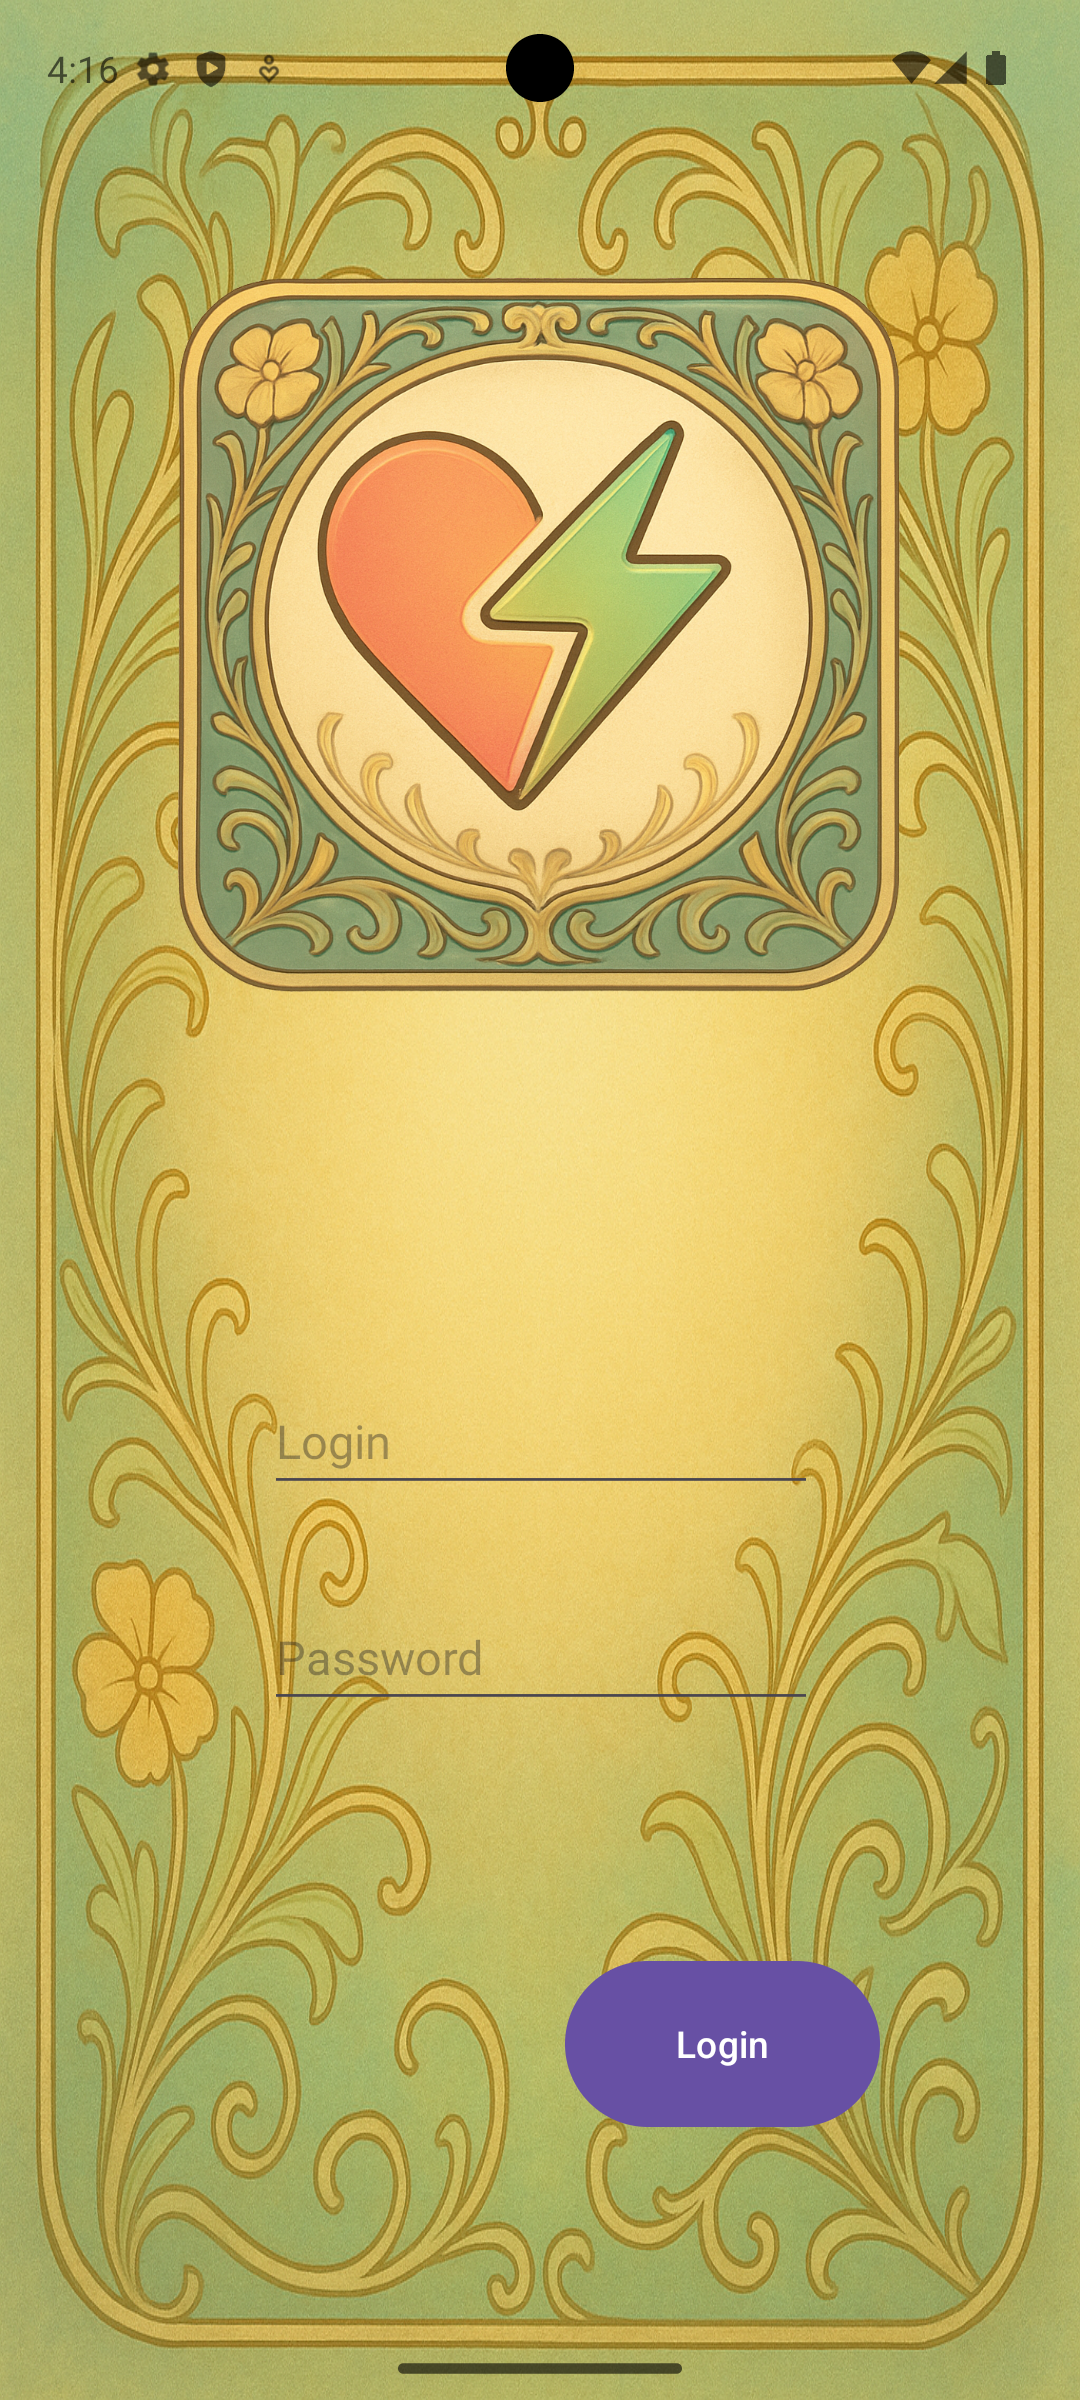
\includegraphics[scale=0.1]{./pictures/screenshot.png}
\end{figure}